% Unified group research paper for MAAI 901 (Deep Learning for Visual Data) and MAAI 902 (NLP & LLMs).
% IEEE conference format. Upload this folder (with figures/) to Overleaf and compile with pdfLaTeX.
\documentclass[conference]{IEEEtran}
\IEEEoverridecommandlockouts
\usepackage{cite}
\usepackage{amsmath,amssymb}
\usepackage{graphicx}
\usepackage{booktabs}
\usepackage{url}
\usepackage[hidelinks]{hyperref}

\begin{document}

\title{Do Candlestick Charts and SEC Filings Forecast Stock Risk? A Pre-Registered Comparison of Vision Networks, Language Models and Their Fusion}

\author{\IEEEauthorblockN{Krishna Harsha Tangirala, [Group member 2] and [Group member 3]}
\IEEEauthorblockA{\emph{Master of Applied Artificial Intelligence, University of Wollongong in Dubai}, Dubai, United Arab Emirates\\
Code and results: \url{https://github.com/harshatangirala/nexus-alpha-v3-university-of-wollongong-in-dubai}\\
CV data: \url{https://drive.google.com/file/d/1Y7wvfpJcjnmXLP79hHTih-jj5pt-muu-/view}\\
NLP data: \url{https://drive.google.com/drive/folders/1nczPvpd_wkMgF5N7uFBfAQMp-Ja96TRI}\\
Lite dashboard (public): \url{https://nexus-alpha-v3-lite.streamlit.app}\\
Full dashboard (heavy): \url{https://buffalo-deposits-graph-legends.trycloudflare.com}}}

\maketitle

\begin{abstract}
Finance apps now claim that deep networks can read price charts and company filings and say what a stock will do next. We tested that claim under conditions designed to prevent false positives. For 50 large US stocks we rendered weekly, daily and hourly candlestick charts (64,550 decision days, 193,650 images) and collected 10,269 SEC filings with point-in-time acceptance stamps. Seven vision networks, from a CNN trained from scratch to ViT-B/16, Swin-T and YOLOv8, and seven text models, from TF-IDF to Longformer and a 4-bit FinGPT-7B, forecast direction, log realised volatility and the risk of a fall of more than 10\% at 5, 10, 20 and 40 trading sessions. All choices were hashed and frozen before a locked test covering January 2024 to August 2026 was opened. Charts carry a small, statistically supported direction signal (about +0.03 macro-F1 over a shuffled-label null at 5 and 10 sessions) and rank drawdown risk above chance. Text models also rank drawdown risk, but lose that edge against a baseline that knows the company and simple price features, because they mostly learn who filed and when. Filing days still move prices about twice as much as matched ordinary days, and filing text explains the size of the reaction beyond company identity (+0.043 $R^2$). Late fusion beats the better single modality in 6 of 12 tasks, and the deployed recipe beats its uninformed benchmark in 9 of 12. Numerical baselines stay stronger on volatility and drawdown, a gap we trace to per-chart price scaling.
\end{abstract}

\begin{IEEEkeywords}
candlestick charts, vision transformers, financial NLP, SEC filings, large language models, multimodal fusion, look-ahead bias, event study
\end{IEEEkeywords}

\section{Introduction}

Retail investors look at candlestick charts every day, and the tools they use now advertise artificial intelligence that spots patterns in those charts. A second wave of products reads company filings with large language models and turns the words into trading signals. Both claims are easy to make and hard to check. A model can look accurate for many reasons that have nothing to do with the chart or the text: the test period may overlap with training, a language model may have read the future during pre-training, or the model may simply learn that some companies are more volatile than others.

The research record has the same weak spots. Jiang, Kelly and Xiu showed that a convolutional network trained on price images predicts US returns \cite{jkx2023}, and earlier work applied CNNs to bar charts \cite{sezer2019}, but most of this literature uses one architecture and one target. Text studies have moved from word lists \cite{tetlock2007,loughran2011} to transformers \cite{araci2019,huang2023finbert} and large language models \cite{lopezlira2023}, yet several of them test on periods the language model may already have seen \cite{glasserman2023,sarkar2024}, and few separate what a filing says from who filed it and when.

This paper puts charts and filings through the same test. We fixed one universe of 50 stocks, one set of twelve targets (direction, volatility and drawdown risk, each at four horizons), one time split and one locked test period, and we compared seven vision networks, seven text models and their fusion on exactly the same rows. We asked four questions:

\begin{enumerate}
\item RQ1. Do vision networks reading multi-timeframe candlestick charts forecast direction, volatility and drawdown risk better than uninformed benchmarks and simple numerical baselines?
\item RQ2. Do SEC filings move prices, and can language models forecast from filing text once company identity and the filing calendar are controlled for?
\item RQ3. Does combining charts and text beat the better of the two on its own?
\item RQ4. Can the result be served in a usable tool that explains its forecasts without overstating them?
\end{enumerate}

The short answers are yes but modestly for charts, a clear yes for the market effect of filings and mostly no for forecasting from text alone, yes for fusion on risk targets, and yes for deployment. The rest of the paper explains how we reached these answers and where they stop. Section II reviews related work, Section III states our contributions, Section IV describes the method, Section V reports ablations, Section VI gives the locked-test results, Section VII discusses limitations and ethics, and Section VIII concludes.

\section{Literature Review}

\subsection{Price images and vision models}

Image-based forecasting began with CNNs trained on stock bar charts \cite{sezer2019}. The large study by Jiang et al. \cite{jkx2023} trained CNNs on millions of simple price images and found a return signal that was strongest for small firms and short horizons. Ho and Huang paired candlestick images with sentiment features \cite{ho2021}. These studies use one network family, so they cannot tell whether a newer architecture reads charts better.

The architectures we compare cover the main ideas of the last decade. ResNet added residual connections \cite{he2016}, EfficientNet scales depth, width and resolution together \cite{tan2019}, and ConvNeXt brings transformer-era design choices back into a convolutional network \cite{liu2022convnext}. The Vision Transformer splits an image into $16\times16$ patches and applies global attention \cite{dosovitskiy2021}, while Swin restricts attention to shifted local windows \cite{liu2021swin}. YOLO was designed for real-time object detection \cite{redmon2016}; its YOLOv8 classification backbone \cite{jocher2023} is a natural candidate because traders describe chart patterns as objects. Charts are an unusual domain for ImageNet-pretrained models: they are synthetic, nearly texture-free and carry their information in geometry and scale. Work on corruption robustness \cite{hendrycks2019} and on probability calibration \cite{guo2017} shaped how we tested and calibrated these models.

\subsection{Text, filings and returns}

Tetlock showed that the tone of a newspaper column predicts market moves \cite{tetlock2007}. Loughran and McDonald built a finance-specific word list after finding that general dictionaries misread 10-K language \cite{loughran2011}, and later surveyed the field \cite{loughran2016}. Lerman and Livnat documented price reactions to the expanded 8-K items introduced in 2004 \cite{lerman2010}, and Cohen, Malloy and Nguyen found that firms that change the wording of their annual reports later underperform \cite{cohen2020}. Ke, Kelly and Xiu learned sentiment directly from returns \cite{kkx2019}.

Transformers \cite{vaswani2017} and BERT \cite{devlin2019} changed the toolkit. FinBERT adapts BERT to financial sentiment \cite{araci2019,huang2023finbert}, SEC-BERT is pre-trained on filings \cite{loukas2022}, RoBERTa and DeBERTa-v3 improve the pre-training recipe at larger sizes \cite{liu2019roberta,he2023deberta}, and Longformer uses sparse attention to read long documents \cite{beltagy2020}. Large generative models such as Llama 2 \cite{touvron2023} can be adapted cheaply with LoRA \cite{hu2022lora} and QLoRA \cite{dettmers2023}, which is how FinGPT is built \cite{yang2023fingpt}. Lopez-Lira and Tang reported that ChatGPT's reading of headlines predicts next-day returns \cite{lopezlira2023}, while Glasserman and Lin \cite{glasserman2023} and Sarkar and Vafa \cite{sarkar2024} warned that such results can come from the model having seen the outcome during pre-training. Grounding a generative model in supplied documents, known as retrieval-augmented generation \cite{lewis2020rag}, is the standard way to keep its answers tied to facts.

\subsection{Fusion and evaluation}

Multimodal learning combines inputs either early, by joining features, or late, by combining each model's outputs \cite{baltrusaitis2019}. Finance adds two evaluation problems. Models can take shortcuts \cite{geirhos2020}, for example learning a company's identity instead of the content of its filing. Fine-tuning large encoders on small, noisy datasets is unstable across seeds \cite{dodge2020,mosbach2021}. Daily returns are dependent, so confidence intervals need a block bootstrap \cite{kunsch1989}, and many simultaneous tests need a family-wise correction such as Holm's \cite{holm1979}. Volatility forecasts should be judged against a proxy and a strong benchmark, usually the HAR model \cite{patton2011,corsi2009}.

We have not found a study that compares modern vision and language families on the same stocks, targets and locked test period while controlling for company identity and the filing calendar, and this paper sets out to do that.

\section{Contributions}

\begin{itemize}
\item A leakage-controlled benchmark: 50 stocks, 64,550 decision days, 193,650 rendered charts and 10,269 point-in-time filings, with twelve targets, a 40-session purge between time blocks and a locked test opened once after a hashed freeze.
\item The first head-to-head comparison, to our knowledge, of seven vision families (CNN, ResNet, EfficientNet, ConvNeXt, ViT, Swin, YOLOv8) on multi-timeframe candlestick charts, showing a small but significant direction signal and a measurable cost of per-chart scaling.
\item A filing study that pairs an event study with seven text models, from TF-IDF to a 7B financial LLM, and uses company and calendar controls to show that most of the apparent text signal is shortcut learning, while the text still explains the size of the market reaction.
\item Evidence that late fusion of charts and text helps on volatility and drawdown risk, with a decomposition of where the gain comes from.
\item A deployed system: a Streamlit dashboard that reads TradingView screenshots, redraws them in the training format, produces a calibrated Monte Carlo price cone and explains each result through a grounded LLM assistant. Code, result tables, data and a public demo are released.
\end{itemize}

\section{Methodology}

\subsection{Universe and data}

The universe holds 50 large US stocks, ten in each of five sectors: Information Technology, Financials, Health Care, Consumer Discretionary and Communication Services. Balancing the sectors stops any one of them from dominating the pooled metrics and lets us test whether model rankings depend on the sector. Hourly, daily and weekly bars were built from a public 1-minute dataset, corrected for five stock-split dates and gap-filled from Yahoo Finance; a SHA-256 manifest pins the exact files.

Filings were downloaded from SEC EDGAR under its fair-access policy (declared user agent, at most eight requests per second). The corpus holds 554 10-Ks, 1,700 10-Qs and 8,015 8-Ks. Each filing's acceptance time comes from its SGML header, and a filing becomes usable 35 minutes after acceptance, at the first hourly bar after that moment. Labels are measured from that entry price.

\subsection{Targets and splits}

One row is one stock on one decision day. For each horizon $h \in \{5,10,20,40\}$ sessions we predict three things. Direction is DOWN, SIDEWAYS or UP, where SIDEWAYS means the log return $r_h$ stays inside a band scaled by the stock's own trailing daily volatility $\sigma$:
\begin{equation}
|r_h| \le 0.5\,\sigma\sqrt{h}.
\end{equation}
Volatility is the log of realised volatility over the window, computed from hourly bars. Drawdown is 1 if the price falls more than 10\% below the decision-day close at any point in the window. Filing models use the same twelve targets measured from the filing entry time.

Data were split by time (Table~\ref{tab:split}) with a 40-session purge between blocks, so no label window crosses into the next block. The 2021 block is used only for early stopping and calibration. All modelling choices were made on validation, written to a registry and hashed before the test was opened.

\begin{table}[t]
\caption{Time blocks, chart rows and filing events}
\label{tab:split}
\centering
\begin{tabular}{lrr}
\toprule
Block & Chart rows & Filing events \\
\midrule
Train, Oct 2016 to Dec 2020 & 51,250 & 4,149 \\
Inner, 2021 (early stopping) & 2,150 & used for stopping \\
Validation, 2022--2023 & 4,600 & 1,529 \\
Locked test, Jan 2024 to Aug 2026 & 6,550 & 2,165 \\
\bottomrule
\end{tabular}
\end{table}

\subsection{Chart representation}

We drew the charts with our own renderer, so every image follows one exact format (Fig.~\ref{fig:charts}). The weekly view shows 52 candles, the daily view 63 and the hourly view 70, each with a volume strip, in a five-colour palette with no axes, dates or text. Each chart is scaled vertically to its own high and low. Images are $224\times224$ pixels and are stored as palette indices, which kept all 193,650 images in 9.72 GB. Augmentation respects what a chart means: no flips, since a horizontal flip reverses time and a vertical flip turns a rally into a crash, only a small vertical rescale, cropping of the oldest bars, brightness changes and Gaussian noise.

\begin{figure}[t]
\centering
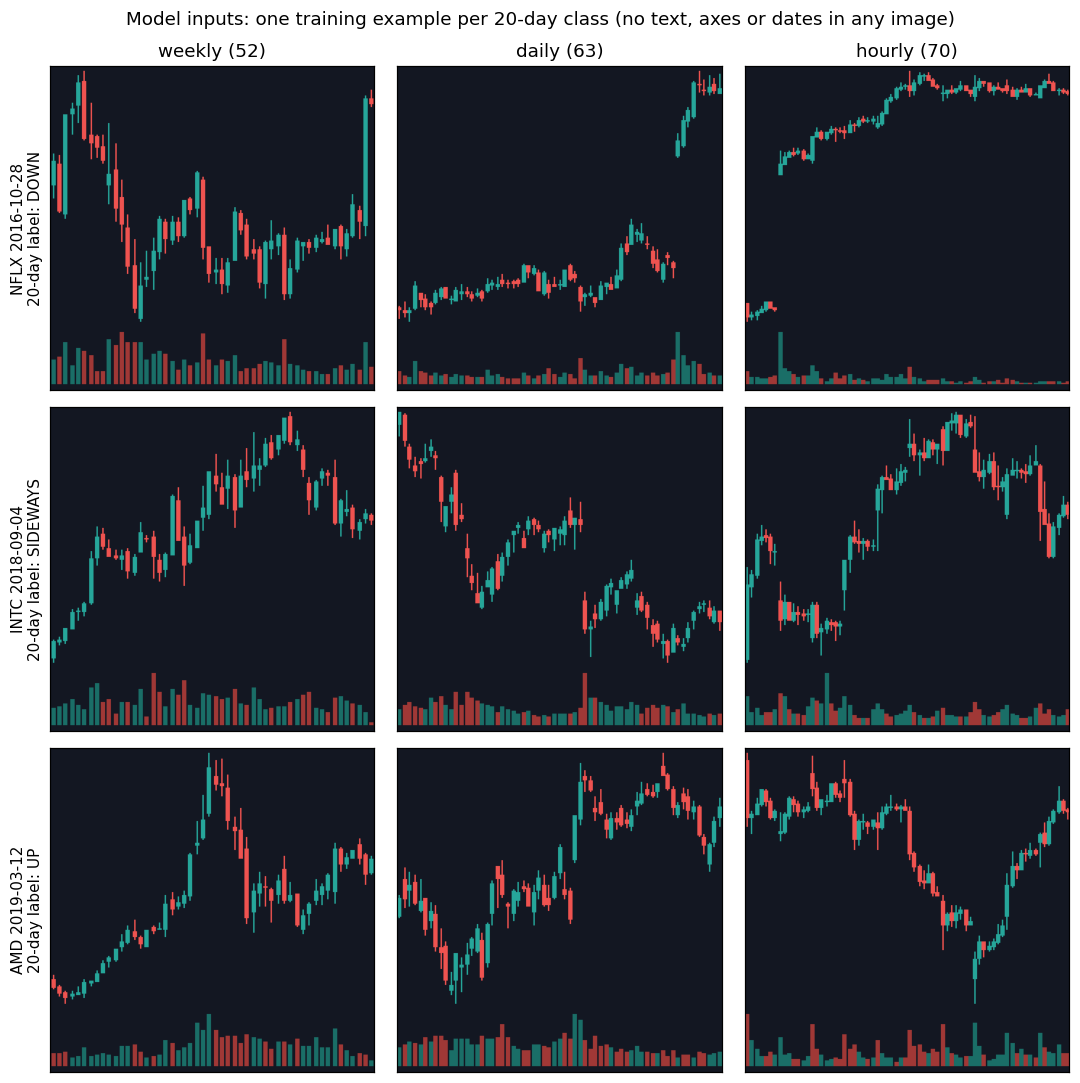
\includegraphics[width=\columnwidth]{figures/chart_gallery.png}
\caption{Model inputs for three training rows, one per 20-session direction class; each row stacks the weekly, daily and hourly charts.}
\label{fig:charts}
\end{figure}

\subsection{Text representation}

For 10-K and 10-Q reports we extracted Management's Discussion and Analysis (MD\&A), the section where managers explain results in their own words; it was found in 85.0\% of 10-Ks and 89.3\% of 10-Qs, and the full document was used otherwise. For 8-Ks we used the body plus the EX-99 press release. Every input starts with its form and section, for example ``[10-Q] [MD\&A]''. Length is a real constraint: the median MD\&A section of a 10-K has 83,366 characters, roughly 20,000 tokens.

\subsection{Models}

Table~\ref{tab:models} lists the fourteen models. All vision networks share one wrapper: a single backbone reads the three timeframes separately, the three feature vectors are concatenated, and a multi-task head (layer normalisation, dropout 0.2 and a 512-unit GELU layer) outputs, for each horizon, three direction logits, one volatility value and one drawdown logit. The custom CNN follows the Jiang et al. design \cite{jkx2023} and is trained from scratch as the academic baseline; the other backbones start from ImageNet weights. The encoders on the text side end in the same head. Each encoder is used in two ways: fine-tuned end to end on the first 512 tokens (4,096 for Longformer), and frozen, with the hidden states of four 512-token chunks mean-pooled, reduced to 32 principal components and fed to regularised linear heads. FinGPT, a LoRA adapter on Llama-2-7B, is loaded in 4-bit precision and used frozen.

\begin{table}[t]
\caption{Models compared and their size}
\label{tab:models}
\centering
\begin{tabular}{llr}
\toprule
Branch & Model & Params (M) \\
\midrule
Vision & Custom CNN, scratch & 3.4 \\
Vision & ResNet-50 & 26.7 \\
Vision & EfficientNet-B0 & 6.0 \\
Vision & ConvNeXt-Tiny & 29.0 \\
Vision & ViT-B/16 & 87.0 \\
Vision & Swin-T & 28.7 \\
Vision & YOLOv8s-cls & 7.1 \\
Text & TF-IDF + linear & 0.75 \\
Text & FinBERT & 109.9 \\
Text & SEC-BERT & 109.5 \\
Text & RoBERTa-large & 355.9 \\
Text & DeBERTa-v3-large & 434.5 \\
Text & Longformer-4096 & 149.1 \\
Text & FinGPT (Llama-2-7B, 4-bit) & 6,738 \\
\bottomrule
\end{tabular}
\end{table}

\subsection{Fusion and deployment}

Fusion is late: each branch is calibrated on its own, the three best models per target on validation are averaged within each branch, and the two averages are blended with a weight chosen per target on validation. Text exists only near filings, so on the daily panel each day sees the most recent filing. Validation gave text no weight for direction and all of the weight for drawdown at 10, 20 and 40 sessions. The dashboard runs a lighter recipe: the top-3 chart ensemble, blended with the three best deployable text models (encoders up to 600 million parameters, or TF-IDF) when the stock filed in the last five sessions. Its 20-session forecasts drive a Monte Carlo cone of 4,000 paths with normal daily shocks, widened by a factor of 1.25; both the shock distribution (Student-$t$ shocks were tried) and the width were chosen on validation.

Users paste TradingView screenshots. The app reads the price axis and candles from the pixels, redraws the three charts in the training format and runs the networks; on 66 real screenshots the median price error was 0.08\%. An assistant built on Google Gemini answers questions about each result. It is grounded: every request carries answering rules, a fact sheet of verified study results, the model routing for each target and the numbers of the current analysis. Fig.~\ref{fig:arch} summarises the pipeline.

\begin{figure*}[t]
\centering
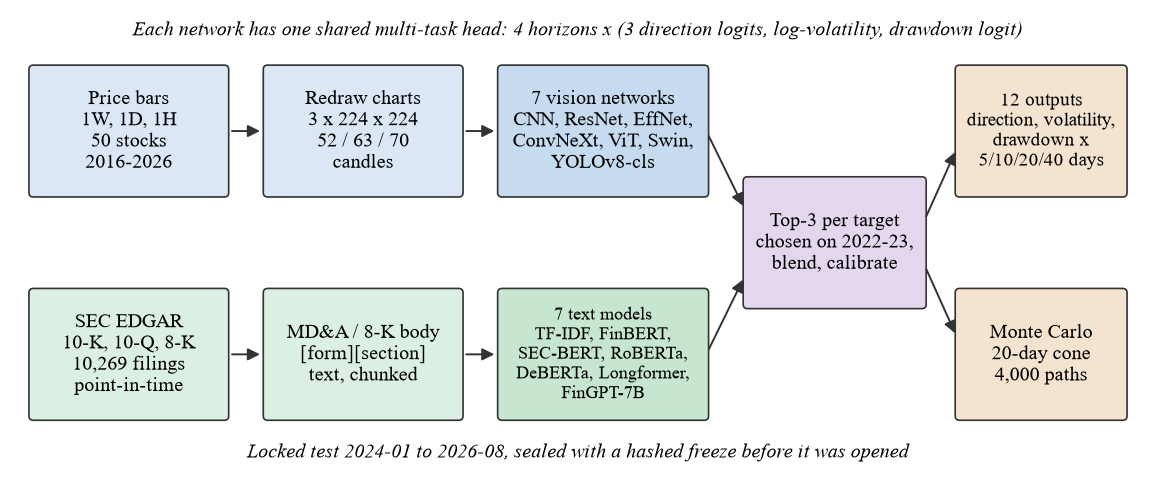
\includegraphics[width=0.9\textwidth]{figures/fig_architecture.png}
\caption{System overview. Chart and text branches share the targets, splits and multi-task head, are calibrated separately and are combined late. The lower right box is the Monte Carlo price cone shown in the dashboard.}
\label{fig:arch}
\end{figure*}

\subsection{Baselines}

Uninformed benchmarks set the floor: the class prior, a volatility forecast equal to the training mean, an AUC of 0.5, and for direction a null model that shuffles labels within each month, which keeps class shares and breaks the link to the future. Numbers-only baselines set a harder bar. \texttt{baseline\_simple} uses momentum for direction, the HAR model \cite{corsi2009} for volatility and a trailing-volatility logistic model for drawdown; \texttt{tech\_gbm} is a LightGBM model on 20 technical indicators. For filings we added three no-text baselines on the same events: per-company base rates, momentum and trailing volatility plus the form, and the technical model plus the form. On the daily panel we also built controls that add only the filing calendar (distance to the last and next filing) and the company identity.

\subsection{Training and calibration}

All models were trained with AdamW, a warm-up followed by cosine decay and mixed precision. Vision networks ran for at most six epochs and text encoders for at most three, with early stopping on 2021. A short probe on a subsample of the training block chose between two learning rates per model. Outputs were calibrated on 2021 only: temperature scaling for direction \cite{guo2017}, Platt scaling for drawdown and a linear map for volatility. The confirmatory run used about 4.2 GPU-hours on one data-centre GPU in Google Colab.

\subsection{Evaluation protocol}

Direction is scored by macro-F1, since always predicting SIDEWAYS already reaches about 42\% accuracy. Direction skill is macro-F1 minus that of the shuffled null. Volatility uses $R^2$ against the training mean and drawdown uses ROC-AUC. Intervals come from a paired month-block bootstrap \cite{kunsch1989}, and each family of tests is Holm-corrected \cite{holm1979}. Eight hypothesis families were registered before the test was opened (H1 to H7, with H2 on filing events and H2b on the daily panel), and the dashboard recipe was scored the same way. Comparisons against the numerical baselines and the calendar and company controls were added after the test was opened and are labelled post-hoc.

\subsection{Design decisions and alternatives}

Table~\ref{tab:alts} lists the main choices, the alternative we considered and why we did not take it.

\begin{table*}[t]
\caption{Design decisions, alternatives considered and the reason for each choice}
\label{tab:alts}
\centering
\begin{tabular}{lll}
\toprule
Decision & Alternative considered & Reason for the choice \\
\midrule
Own chart renderer & Broker screenshots for training & Screenshots vary in theme, axes and fonts; a renderer gives one format and byte-exact reruns \\
Per-chart vertical scaling & Fixed scale across stocks & Keeps the shape of the path comparable; costs the volatility level (Section V) \\
Volatility-scaled sideways band & Fixed percentage threshold & A fixed band labels volatile stocks almost always UP or DOWN \\
Time blocks with 40-session purge & Random k-fold & Random folds let overlapping label windows leak across splits \\
Macro-F1 over a shuffled null & Accuracy & Accuracy rewards always predicting SIDEWAYS \\
MD\&A and 8-K press release & Full 10-K text & A full 10-K is far beyond any context window; MD\&A carries management's own account \\
Frozen 4-bit FinGPT & QLoRA fine-tuning & GPU budget; QLoRA is the first item of the follow-up protocol \\
Late fusion & Early fusion on joint features & Text is missing on most days; early fusion trailed on direction and volatility \\
Grounded full-context prompt & Vector-index RAG & The knowledge base is a few pages, so the whole of it fits in every request \\
\bottomrule
\end{tabular}
\end{table*}

\section{Ablation Studies}

Ablations were run on validation with 5,000 paired bootstrap draws, except where we say test.

\subsection{Vision branch}

The vertical-rescale augmentation turned out to be the most consequential choice. Removing it changed volatility $R^2$ by 0.135 in favour of the un-augmented model, and per-chart scaling hides the absolute size of the candles: a chart that always fills its frame cannot show a calm month as calm. On the test, fine-tuning beat frozen features in 9 of 18 network-target tests; ConvNeXt-T, ViT-B/16 and Swin-T gained most, while EfficientNet-B0 got worse on all three targets. ImageNet initialisation beat random initialisation for ResNet-50 on direction (+0.035 macro-F1). Occlusion showed that the weekly chart moves predictions most and the hourly chart least. A light-theme rendering lowered ResNet-50's 20-session macro-F1 by 0.16, while JPEG compression, blur and noise changed little; this is why the dashboard redraws every screenshot instead of feeding it in raw.

\subsection{Language branch}

Reading four chunks instead of the first 512 tokens helped frozen encoders on risk targets, for example +0.140 drawdown AUC for RoBERTa-large and +0.101 for SEC-BERT. Length helped Longformer against FinBERT on drawdown (+0.115 AUC). Domain pre-training helped SEC-BERT against FinBERT on direction (+0.067 macro-F1) but cost 0.148 of volatility $R^2$. Fine-tuning against frozen features was mixed: +0.084 AUC for Longformer on drawdown and $-0.034$ macro-F1 for FinBERT on direction. DeBERTa-v3-large was unstable, with a best early-stopping loss of 1.91 against 1.44 to 1.52 for the other encoders, which matches known fine-tuning instability at this data size \cite{dodge2020,mosbach2021}.

\subsection{Ensembles}

On the test, combinations of two or three vision networks beat the best single network in 5 of 12 tasks and lost in none. Combinations of language models never beat the best single one (0 of 12), which suggests their errors overlap. Adding the text combination to the chart combination improved drawdown at 20 and 40 sessions (+0.090 and +0.061 AUC) and left the other ten tasks level.

\subsection{Where the fusion gain comes from}

Adding chart and text outputs to the technical model improved it in 6 of 12 test tasks and hurt it in 2. We decomposed this gain with nested controls (Table~\ref{tab:hyp}). Charts alone added a little to volatility (3 tasks, +0.004 to +0.026 $R^2$). Text added more: volatility $R^2$ rose by 0.075 on average. The filing-calendar columns alone, without any text, produced 0.063 of that gain. The words added 0.013 beyond the calendar and 0.007 beyond the calendar and the company. Integrated-gradients attributions \cite{sundararajan2017} for the largest reactions were dominated by dates, company names and formatting tokens. The text models had mostly learned when and by whom a filing was made.

\section{Results}

\subsection{Confirmatory tests}

Table~\ref{tab:hyp} collects the hypothesis families. Charts showed skill in 6 of 12 tasks (H1): direction at 5 and 10 sessions, volatility at 5 sessions and drawdown at 5, 10 and 40 sessions. Text showed skill in 4 of 12 on filing events (H2), all of them drawdown. Fusion beat the better single modality in 6 of 12 (H3): all four volatility horizons, by $+0.053$ to $+0.159$ $R^2$, and drawdown at 5 and 40 sessions. Model rankings depended on the sector for volatility and drawdown (permutation $p = 0.015$ and $0.005$) but not for direction. The recipe the dashboard runs beat its uninformed benchmark in 9 of 12 tasks.

\begin{table}[t]
\caption{Locked-test hypothesis families (Holm-corrected)}
\label{tab:hyp}
\centering
\begin{tabular}{lll}
\toprule
ID & Comparison & Result \\
\midrule
H1 & Charts vs uninformed benchmark & 6 of 12 \\
H2 & Text vs uninformed (filing events) & 4 of 12 \\
H3 & Fusion vs better single modality & 6 of 12 \\
H4 & Top-3 + top-3 vs top-3 charts & 3 of 12 \\
H5 & Fine-tuned vs frozen & 9 of 18 \\
H6 & Sector-dependent rankings & 2 of 3 \\
H7 & Filings move prices & 2 of 2 \\
Deploy & Dashboard recipe vs uninformed & 9 of 12 \\
H1c & Charts vs numbers-only & 4 better, 8 worse \\
H2c & Text vs no-text, same filings & 1 better, 7 level, 4 worse \\
H3c & Fusion vs numbers-only & 4 better, 1 level, 7 worse \\
H8 & Technical + charts + text vs technical & 6 better, 4 level, 2 worse \\
H8d & Technical + calendar vs technical & 6 better, 6 level \\
H8f & Text beyond calendar and company & 1 better, 9 level, 2 worse \\
\bottomrule
\end{tabular}
\end{table}

\subsection{Vision results}

ConvNeXt-Tiny was the validation choice for three of the four direction horizons, with test skill of +0.032 (interval 0.019 to 0.043) at 5 sessions and +0.030 (0.015 to 0.046) at 10, and it remained the best direction network in every sector. The gain is small, as one would expect for a three-class label whose band moves with each stock's volatility. Plain accuracy at 5 sessions was 0.416 against 0.420 for always predicting SIDEWAYS, but balanced accuracy was higher by 0.036 on average across horizons: the network catches some of the DOWN and UP moves that a majority-class model never calls. Swin-T reached $R^2 = 0.084$ for 5-session volatility. For drawdown the supported AUCs were 0.605 at 5 sessions (Swin-T), 0.586 at 10 (ResNet-50) and 0.540 at 40 (ViT-B/16).

Rankings shifted between validation and test. ViT-B/16 led on validation and ranked third on the test, behind Swin-T and ConvNeXt-T. Validation held the 2022 bear market (a 20-session drawdown rate of 23.7\%) and the test a strong rally, which is why the deployed system averages the top three networks per target. A ready-made YOLOv8 chart-pattern detector, run zero-shot on the weekly charts, found many head-and-shoulders, double tops and double bottoms, but returns barely differed between rows with and without a pattern (for double bottoms, 0.9\% against 1.5\% over 20 sessions).

\subsection{Filings and the language models}

The event study gives the clearest result in the paper (Fig.~\ref{fig:event}). On filing days the mean absolute abnormal two-day move was 1.43 normal-day units, against 0.70 on matched days without a filing (one-sided Mann-Whitney $p < 0.001$). Forms differ (Kruskal-Wallis $p = 0.006$): quarterly reports move prices most (1.64), then annual reports (1.52) and 8-Ks (1.37). In the development blocks, 8-K item 2.02 (results of operations) produced a mean move of 2.39 over 1,446 filings.

\begin{figure}[t]
\centering
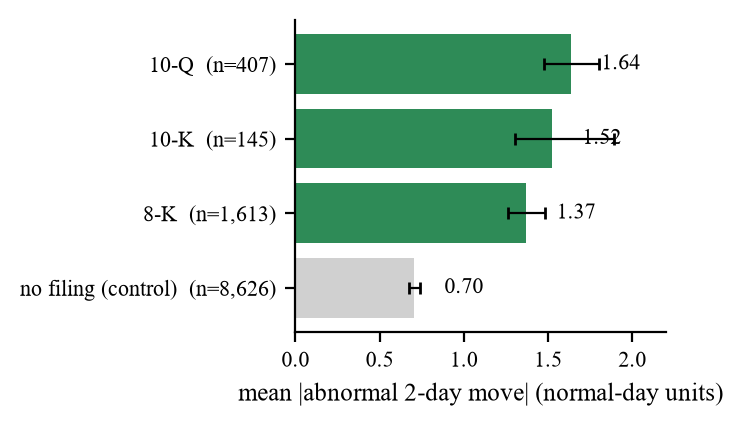
\includegraphics[width=\columnwidth]{figures/fig_event_study_test.png}
\caption{Locked-test event study: mean absolute abnormal two-day move by filing type, with 95\% intervals.}
\label{fig:event}
\end{figure}

Forecasting from the text is much weaker. The validation-chosen text models showed skill only on drawdown, where Longformer reached AUCs of 0.61 to 0.65, and volatility $R^2$ was negative at every horizon. Against the strongest no-text baseline on the same filings, the best text model was better in 1 of 12 tasks (SEC-BERT on 20-session direction, +0.086 macro-F1 over company base rates), level in 7 and worse in 4. The words do explain the size of the reaction. In a regression of the absolute abnormal move on form, 8-K items, sector and timing, TF-IDF features raised $R^2$ from 0.181 to 0.235, and the gain held at +0.043 (0.029 to 0.058) once the company was also controlled for. Interpretable measures added nothing: dictionary tone \cite{loughran2011} and year-on-year text change \cite{cohen2020} did not improve the no-text model, and FinBERT sentence tone had a Spearman correlation of only 0.025 with the signed reaction. On validation TF-IDF had the best mean rank of the seven text models (2.92), and on the test SEC-BERT ranked first (2.58).

\subsection{Against numbers-only baselines}

Table~\ref{tab:main} and Fig.~\ref{fig:bench} set every branch against the baselines. On direction the chart ensemble's macro-F1 is higher than both numerical baselines at every horizon. We do not read this as a large win: the baselines mostly predict one class, which macro-F1 punishes, and a ResNet-50 probe trained on shuffled labels also beat them on macro-F1 in three of four tasks. Judged fairly, with each model scored against its own shuffled null, charts beat the baselines at 5 sessions (+0.024, interval 0.007 to 0.039) and were level at 10, 20 and 40. On volatility and drawdown the order reverses. \texttt{tech\_gbm} reaches $R^2 = 0.371$ at 5 sessions against 0.132 for the chart ensemble, and the simple drawdown model reaches an AUC of 0.693 against 0.620. Adding charts and text to the technical model gives the best volatility forecasts in the study ($R^2 = 0.446$ at 5 and 10 sessions).

\begin{table*}[t]
\caption{Locked-test primary metric per task: macro-F1 for direction, $R^2$ for volatility, ROC-AUC for drawdown}
\label{tab:main}
\centering
\begin{tabular}{lrrrrrrr}
\toprule
Task & Top-3 charts & Top-3 text & Late fusion & Technical + charts + text & \texttt{tech\_gbm} & \texttt{baseline\_simple} & Prior \\
\midrule
Direction 5 & 0.329 & 0.199 & 0.329 & 0.197 & 0.197 & 0.243 & 0.197 \\
Direction 10 & 0.360 & 0.246 & 0.360 & 0.251 & 0.226 & 0.256 & 0.194 \\
Direction 20 & 0.369 & 0.283 & 0.369 & 0.244 & 0.264 & 0.292 & 0.190 \\
Direction 40 & 0.363 & 0.279 & 0.363 & 0.297 & 0.298 & 0.287 & 0.181 \\
Volatility 5 & 0.132 & $-$0.075 & 0.148 & 0.446 & 0.371 & 0.304 & $-$0.069 \\
Volatility 10 & 0.062 & $-$0.090 & 0.085 & 0.446 & 0.352 & 0.308 & $-$0.099 \\
Volatility 20 & 0.010 & $-$0.076 & 0.046 & 0.405 & 0.314 & 0.317 & $-$0.135 \\
Volatility 40 & $-$0.112 & $-$0.079 & $-$0.047 & 0.355 & 0.292 & 0.295 & $-$0.186 \\
Drawdown 5 & 0.620 & 0.612 & 0.637 & 0.710 & 0.701 & 0.693 & 0.500 \\
Drawdown 10 & 0.590 & 0.601 & 0.601 & 0.687 & 0.649 & 0.666 & 0.500 \\
Drawdown 20 & 0.537 & 0.588 & 0.588 & 0.639 & 0.620 & 0.633 & 0.500 \\
Drawdown 40 & 0.518 & 0.586 & 0.586 & 0.575 & 0.602 & 0.590 & 0.500 \\
\bottomrule
\end{tabular}
\end{table*}

\begin{figure*}[t]
\centering
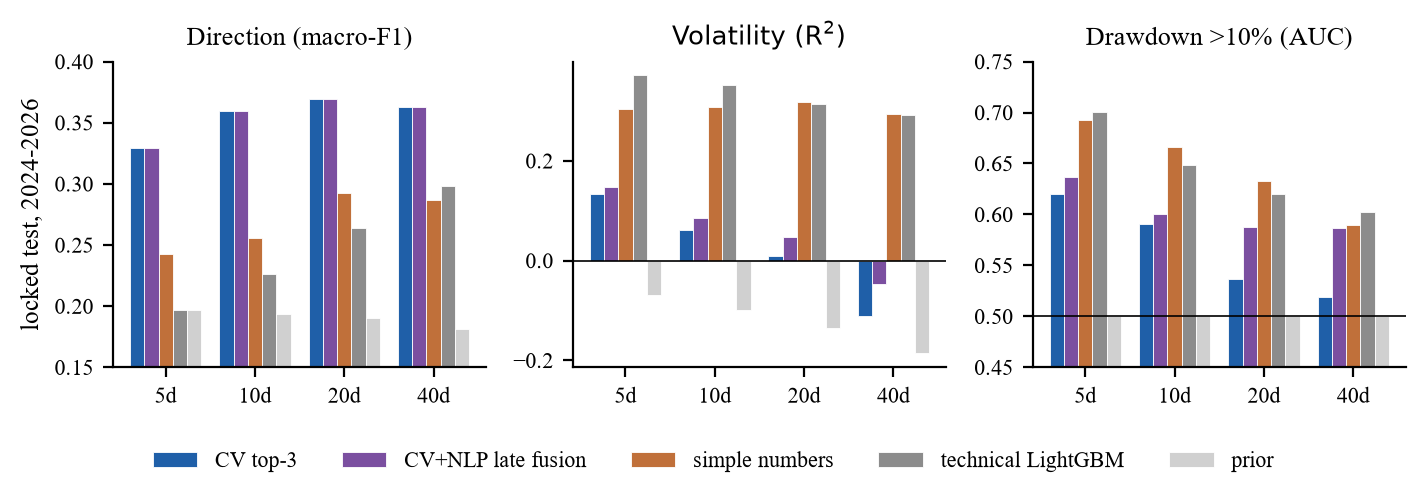
\includegraphics[width=0.85\textwidth]{figures/fig_benchmarks_test.png}
\caption{Locked-test primary metrics for the top-3 chart ensemble, the chart and text fusion, the two numerical baselines and the prior.}
\label{fig:bench}
\end{figure*}

\subsection{Deployment}

The recipe the dashboard runs is the only model in the study judged on all twelve targets as a product. It beat its uninformed benchmark at every direction horizon (+0.023 to +0.036 macro-F1 over the null), at 5-session volatility ($R^2 = 0.140$) and at every drawdown horizon (AUC 0.54 to 0.63). Its Monte Carlo cone was well calibrated: the nominal 80\% and 90\% ranges contained 82.6\% and 90.8\% of realised 20-session returns. Drawdown probabilities rank risk well but set its level poorly (Brier skill between $-0.046$ and $-0.015$ against a constant forecast), so the dashboard labels them as relative risk.

\begin{figure}[t]
\centering
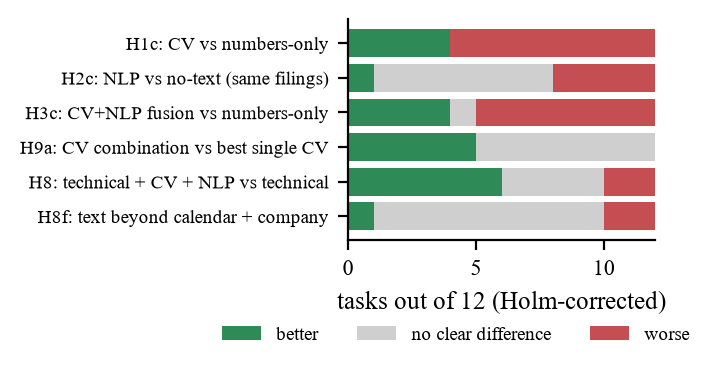
\includegraphics[width=\columnwidth]{figures/fig_hypotheses.png}
\caption{Locked-test comparisons against the strongest baselines and controls, counted over twelve tasks after Holm correction.}
\label{fig:hyp}
\end{figure}

\section{Discussion}

\subsection{What the evidence supports}

The design worked as intended: it found real but small signals and stopped us from reporting larger ones that were not there. Fig.~\ref{fig:hyp} shows the pattern. Charts help with direction at short horizons, where numerical baselines struggle, and they rank drawdown risk above chance. Text helps once it is joined to the charts or to a technical model, mainly for volatility and drawdown. The market effect of filings is large and consistent across sectors, with Communication Services reacting most to quarterly reports and Financials least to 10-Qs and 8-Ks in both development and test. A practitioner should use chart and text models alongside plain numerical features, since on risk targets the numbers still do most of the work.

\subsection{Why charts lose on volatility}

Per-chart scaling is the main reason charts trail \texttt{tech\_gbm} on volatility and drawdown. Every chart fills its frame, so a stock that moved 2\% and one that moved 20\% can produce similar pictures. The ablation shows the cost directly, and the technical model, which sees trailing volatility as a number, does not pay it. This also explains why fusion gains concentrate on risk targets: the text branch and the filing calendar bring information about upcoming volatility that the scaled charts have thrown away. Our follow-up protocol therefore tests a fixed-scale chart encoding.

\subsection{Shortcut learning in text}

A filing reveals the company, and the calendar reveals when earnings are due. Both are predictive of volatility, and neither requires reading. Without the company and calendar controls, our drawdown and volatility results for text would have looked like a genuine language signal. With them, the words add little to forecasting and a clear amount to explaining reaction size. We think this distinction will matter for anyone building LLM products on filings: a model that explains a past reaction well need not forecast the next one.

\subsection{Relation to prior work}

Jiang et al. found most of their image signal in small stocks \cite{jkx2023}; our universe is 50 large, liquid companies, so a modest signal is consistent with their results. Headline-based LLM studies report stronger effects \cite{lopezlira2023}, but they work at a daily horizon on news, and our test starts after every model's pre-training cut-off, which removes the look-ahead channel that Glasserman and Lin describe \cite{glasserman2023}.

\subsection{Limitations}

The universe is small and made of survivors. Each model was trained with one seed, so differences between close models should be read from the intervals, not from ranks. There is one test period, and it was a strong rally, very different from the bear market in validation. FinGPT was used frozen, and DeBERTa-v3-large was not trained to its potential. Macro-F1 against one-class baselines flatters every model, which is why we report skill over each model's own null. Several baseline comparisons were added after the test was opened and are labelled post-hoc.

\subsection{Ethical considerations}

Look-ahead bias is an integrity issue as much as a technical one. The test labels sat in a hashed vault whose openings were logged, every timestamp is point-in-time, and the test period begins after every language model's pre-training cut-off. The text models learned company identity, a form of bias that makes forecasts partly a replay of a company's past; Financials, with almost twice as many 8-Ks as any other sector, also weighed more in training. We report results by sector and the dashboard warns users when a stock lies outside the 50 training companies.

Filings are public records and contain no personal data beyond executive names that companies publish themselves. EDGAR's fair-access rules were respected. The price bars come from a public dataset without a declared licence, which we state openly; we share them for non-commercial academic reproduction only. Pre-trained models are used under their own licences, including the Llama 2 Community License, and no weights are redistributed.

The main risk of harm is misuse by retail investors. The dashboard shows a direction call only where the locked test supported it, labels drawdown as relative risk and states that it is educational research. The LLM assistant can sound more certain than the evidence, so its prompt restricts it to verified results, forbids buy or sell advice and invented numbers, and users are told that questions are sent to Google. Testing found a real failure in an earlier version, which answered several questions with ``this was not tested'' although measured results existed; adding the verified results and the per-target routing to the prompt fixed it. The study used about 4.2 GPU-hours, and later analyses reused cached predictions.

\section{Conclusion}

We compared seven vision networks, seven text models and their fusion on 50 US stocks under a pre-registered, leakage-controlled protocol. Candlestick charts carry a small direction signal at 5 and 10 sessions and rank drawdown risk above chance. Filings roughly double the size of price reactions and their text explains how large a reaction will be, but text alone does not forecast the next move once the company and the calendar are known. Fusion helps on volatility and drawdown, the deployed recipe beats its uninformed benchmark in 9 of 12 tasks, and simple numerical baselines still win on risk because per-chart scaling hides the volatility level.

A pre-registered follow-up will test a fixed-scale chart encoding, five seeds per model, layer-wise learning-rate decay for large encoders, QLoRA fine-tuning of FinGPT and minute-stamped news, on a forward test period that starts in December 2026 and on a wider universe that includes delisted companies.

\section*{Author Contributions and Learning}

Krishna Harsha Tangirala defined the research questions and the two-branch design, chose the seven vision networks, the seven text models, the filing types, the targets and the horizons, ran every Colab execution of the notebook, reviewed each result and audit, decided which post-hoc controls to add and directed the dashboard and its assistant. His main lesson was that controls matter more than model size: the company and calendar baselines changed the conclusion of the text study. [Group member 2: role, contribution and learning.] [Group member 3: role, contribution and learning.]

\section*{Use of Generative AI}

In line with the UOW guidance on acknowledging generative AI, we record that Anthropic's Claude Code wrote most of the code and the Colab notebook and drafted parts of this paper under the first author's direction, and that Google Gemini powers the dashboard assistant. Every number in the paper comes from the executed notebook's output files and was checked against them; no data were generated by an AI tool.

\section*{Data and Code Availability}

Code, notebook, result tables and dashboard: \url{https://github.com/harshatangirala/nexus-alpha-v3-university-of-wollongong-in-dubai}. Price bars for the charts: \url{https://drive.google.com/file/d/1Y7wvfpJcjnmXLP79hHTih-jj5pt-muu-/view}. Filing text and metadata: \url{https://drive.google.com/drive/folders/1nczPvpd_wkMgF5N7uFBfAQMp-Ja96TRI}. All project data: \url{https://drive.google.com/drive/folders/13rokT8OX1MgZQpzTRLeyvDq-FVdgraSh}. The full dashboard loads 13 networks (2.9 GB of weights, about 5 GB of memory), which is too heavy for free hosting, so a lite version is public at \url{https://nexus-alpha-v3-lite.streamlit.app}; the full version runs on the first author's machine during demonstrations at \url{https://buffalo-deposits-graph-legends.trycloudflare.com}.

\begin{thebibliography}{99}

\bibitem{jkx2023} J. Jiang, B. Kelly, and D. Xiu, ``(Re-)Imag(in)ing price trends,'' \emph{The Journal of Finance}, vol. 78, no. 6, pp. 3193--3249, 2023.

\bibitem{sezer2019} O. B. Sezer and A. M. Ozbayoglu, ``Financial trading model with stock bar chart image time series with deep convolutional neural networks,'' \emph{Intelligent Automation \& Soft Computing}, vol. 26, no. 2, pp. 323--334, 2019.

\bibitem{tetlock2007} P. C. Tetlock, ``Giving content to investor sentiment: The role of media in the stock market,'' \emph{The Journal of Finance}, vol. 62, no. 3, pp. 1139--1168, 2007.

\bibitem{loughran2011} T. Loughran and B. McDonald, ``When is a liability not a liability? Textual analysis, dictionaries, and 10-Ks,'' \emph{The Journal of Finance}, vol. 66, no. 1, pp. 35--65, 2011.

\bibitem{araci2019} D. Araci, ``FinBERT: Financial sentiment analysis with pre-trained language models,'' arXiv:1908.10063, 2019.

\bibitem{huang2023finbert} A. H. Huang, H. Wang, and Y. Yang, ``FinBERT: A large language model for extracting information from financial text,'' \emph{Contemporary Accounting Research}, vol. 40, no. 2, pp. 806--841, 2023.

\bibitem{lopezlira2023} A. Lopez-Lira and Y. Tang, ``Can ChatGPT forecast stock price movements? Return predictability and large language models,'' arXiv:2304.07619, 2023.

\bibitem{glasserman2023} P. Glasserman and C. Lin, ``Assessing look-ahead bias in stock return predictions generated by GPT sentiment analysis,'' arXiv:2309.17322, 2023.

\bibitem{sarkar2024} S. K. Sarkar and K. Vafa, ``Lookahead bias in pretrained language models,'' SSRN Working Paper 4754678, 2024.

\bibitem{ho2021} T.-T. Ho and Y. Huang, ``Stock price movement prediction using sentiment analysis and candlestick chart representation,'' \emph{Sensors}, vol. 21, no. 23, p. 7957, 2021.

\bibitem{he2016} K. He, X. Zhang, S. Ren, and J. Sun, ``Deep residual learning for image recognition,'' in \emph{Proc. IEEE CVPR}, 2016, pp. 770--778.

\bibitem{tan2019} M. Tan and Q. Le, ``EfficientNet: Rethinking model scaling for convolutional neural networks,'' in \emph{Proc. ICML}, PMLR 97, 2019, pp. 6105--6114.

\bibitem{liu2022convnext} Z. Liu, H. Mao, C.-Y. Wu, C. Feichtenhofer, T. Darrell, and S. Xie, ``A ConvNet for the 2020s,'' in \emph{Proc. IEEE CVPR}, 2022, pp. 11976--11986.

\bibitem{dosovitskiy2021} A. Dosovitskiy \emph{et al.}, ``An image is worth 16x16 words: Transformers for image recognition at scale,'' in \emph{Proc. ICLR}, 2021.

\bibitem{liu2021swin} Z. Liu \emph{et al.}, ``Swin Transformer: Hierarchical vision transformer using shifted windows,'' in \emph{Proc. IEEE ICCV}, 2021, pp. 10012--10022.

\bibitem{redmon2016} J. Redmon, S. Divvala, R. Girshick, and A. Farhadi, ``You only look once: Unified, real-time object detection,'' in \emph{Proc. IEEE CVPR}, 2016, pp. 779--788.

\bibitem{jocher2023} G. Jocher, A. Chaurasia, and J. Qiu, ``Ultralytics YOLOv8,'' software, 2023. [Online]. Available: \url{https://github.com/ultralytics/ultralytics}

\bibitem{hendrycks2019} D. Hendrycks and T. Dietterich, ``Benchmarking neural network robustness to common corruptions and perturbations,'' in \emph{Proc. ICLR}, 2019.

\bibitem{guo2017} C. Guo, G. Pleiss, Y. Sun, and K. Q. Weinberger, ``On calibration of modern neural networks,'' in \emph{Proc. ICML}, PMLR 70, 2017, pp. 1321--1330.

\bibitem{loughran2016} T. Loughran and B. McDonald, ``Textual analysis in accounting and finance: A survey,'' \emph{Journal of Accounting Research}, vol. 54, no. 4, pp. 1187--1230, 2016.

\bibitem{lerman2010} A. Lerman and J. Livnat, ``The new Form 8-K disclosures,'' \emph{Review of Accounting Studies}, vol. 15, no. 4, pp. 752--778, 2010.

\bibitem{cohen2020} L. Cohen, C. Malloy, and Q. Nguyen, ``Lazy prices,'' \emph{The Journal of Finance}, vol. 75, no. 3, pp. 1371--1415, 2020.

\bibitem{kkx2019} Z. T. Ke, B. T. Kelly, and D. Xiu, ``Predicting returns with text data,'' NBER Working Paper 26186, 2019.

\bibitem{vaswani2017} A. Vaswani \emph{et al.}, ``Attention is all you need,'' in \emph{Advances in Neural Information Processing Systems}, vol. 30, 2017, pp. 5998--6008.

\bibitem{devlin2019} J. Devlin, M.-W. Chang, K. Lee, and K. Toutanova, ``BERT: Pre-training of deep bidirectional transformers for language understanding,'' in \emph{Proc. NAACL-HLT}, 2019, pp. 4171--4186.

\bibitem{loukas2022} L. Loukas \emph{et al.}, ``FiNER: Financial numeric entity recognition for XBRL tagging,'' in \emph{Proc. ACL}, 2022, pp. 4419--4431.

\bibitem{liu2019roberta} Y. Liu \emph{et al.}, ``RoBERTa: A robustly optimized BERT pretraining approach,'' arXiv:1907.11692, 2019.

\bibitem{he2023deberta} P. He, J. Gao, and W. Chen, ``DeBERTaV3: Improving DeBERTa using ELECTRA-style pre-training with gradient-disentangled embedding sharing,'' in \emph{Proc. ICLR}, 2023.

\bibitem{beltagy2020} I. Beltagy, M. E. Peters, and A. Cohan, ``Longformer: The long-document transformer,'' arXiv:2004.05150, 2020.

\bibitem{touvron2023} H. Touvron \emph{et al.}, ``Llama 2: Open foundation and fine-tuned chat models,'' arXiv:2307.09288, 2023.

\bibitem{hu2022lora} E. J. Hu \emph{et al.}, ``LoRA: Low-rank adaptation of large language models,'' in \emph{Proc. ICLR}, 2022.

\bibitem{dettmers2023} T. Dettmers, A. Pagnoni, A. Holtzman, and L. Zettlemoyer, ``QLoRA: Efficient finetuning of quantized LLMs,'' in \emph{Advances in Neural Information Processing Systems}, vol. 36, 2023.

\bibitem{yang2023fingpt} H. Yang, X.-Y. Liu, and C. D. Wang, ``FinGPT: Open-source financial large language models,'' arXiv:2306.06031, 2023.

\bibitem{lewis2020rag} P. Lewis \emph{et al.}, ``Retrieval-augmented generation for knowledge-intensive NLP tasks,'' in \emph{Advances in Neural Information Processing Systems}, vol. 33, 2020, pp. 9459--9474.

\bibitem{baltrusaitis2019} T. Baltrušaitis, C. Ahuja, and L.-P. Morency, ``Multimodal machine learning: A survey and taxonomy,'' \emph{IEEE Transactions on Pattern Analysis and Machine Intelligence}, vol. 41, no. 2, pp. 423--443, 2019.

\bibitem{geirhos2020} R. Geirhos \emph{et al.}, ``Shortcut learning in deep neural networks,'' \emph{Nature Machine Intelligence}, vol. 2, no. 11, pp. 665--673, 2020.

\bibitem{dodge2020} J. Dodge, G. Ilharco, R. Schwartz, A. Farhadi, H. Hajishirzi, and N. Smith, ``Fine-tuning pretrained language models: Weight initializations, data orders, and early stopping,'' arXiv:2002.06305, 2020.

\bibitem{mosbach2021} M. Mosbach, M. Andriushchenko, and D. Klakow, ``On the stability of fine-tuning BERT: Misconceptions, explanations, and strong baselines,'' in \emph{Proc. ICLR}, 2021.

\bibitem{kunsch1989} H. R. Künsch, ``The jackknife and the bootstrap for general stationary observations,'' \emph{The Annals of Statistics}, vol. 17, no. 3, pp. 1217--1241, 1989.

\bibitem{holm1979} S. Holm, ``A simple sequentially rejective multiple test procedure,'' \emph{Scandinavian Journal of Statistics}, vol. 6, no. 2, pp. 65--70, 1979.

\bibitem{patton2011} A. J. Patton, ``Volatility forecast comparison using imperfect volatility proxies,'' \emph{Journal of Econometrics}, vol. 160, no. 1, pp. 246--256, 2011.

\bibitem{corsi2009} F. Corsi, ``A simple approximate long-memory model of realized volatility,'' \emph{Journal of Financial Econometrics}, vol. 7, no. 2, pp. 174--196, 2009.

\bibitem{sundararajan2017} M. Sundararajan, A. Taly, and Q. Yan, ``Axiomatic attribution for deep networks,'' in \emph{Proc. ICML}, PMLR 70, 2017, pp. 3319--3328.

\end{thebibliography}

\end{document}
